\section{Versuch 5: Modulator}\label{sec:modulator}
	\develnote{Wieder ein einfacher Multiplexer, diesmal lassen wir allerdings die gesamte entity und architecture programmieren. Die Studies sollen ja schlie�lich VHDL lernen. Auch in MATLAB werden jetzt keine Strukturen mehr vorgegeben. Die Studenten sollen jetzt ihre Skripten / Funktionen selbst erstellen.}

\subsection{Konzept}\label{subsec:modulator:concept}

Die �bertragung von Daten �ber eine beliebige �bertragungsstrecke ist nicht ohne weiteres (fehlerfrei) m�glich. W�rde man die Daten 1:1 �ber den Kanal schicken, das hei�t zum Beispiel durch Codierung der Null-Bits mit einer Spannung von 0 Volt und der Eins-Bits mit 3.3 Volt, w�re das Ergebnis ziemlich ern�chternd. Kleinere Spannungsschwankungen wirken sich in diesem Fall direkt auf das Empfangssignal aus. Um hier Fehler schon im Vorfeld auszuschlie�en wird das Signal vor der �bertragung moduliert, wodurch die St�ranf�lligkeit verringert wird.

\subsection{Realisierungsm�glichkeiten}\label{subsec:modulator:possibilities}

Um das Praktikum nicht zu kompliziert zu gestalten werden wir uns mit einer einfachen FSK-Modulation\footnote{Frequency Shift Keying}\index{FSK-Modulation} begn�gen. Hierbei werden Nullen und Eisen durch zwei Sinusschwingungen unterschiedlicher Frequenz dargestellt. F�r eine logische Null wird die eine, f�r eine Eins die andere Frequenz �bertragen. Sie haben im Verlauf der ersten Kapitel die n�tigen Baugruppen bereits kennengelernt. Nun werden sie den kompletten FSK-Sender, wie im Blockschaltbild in Abb. \ref{abb:sender_blockschaltbild2}, aufbauen.

\begin{figure}[ht]
	\centering 
	%\psfrag{01}{MATLAB Workspace}
	\includegraphics[width=10cm]{bilder/sender/sender_blockschaltbild}
	\caption{Sender Blockschaltbild}
	\label{abb:sender_blockschaltbild2}\index{Sender Blockschaltbild}
\end{figure}

\subsection{MATLAB: Programmierung}\label{subsec:modulator:matlab}

\paragraph{Aufgabe 1:}
Schreiben sie ein MATLAB-Skript, das unter Verwendung der bisher programmierten Funktionen \textit{PRNseq.m}, \textit{cordic.m} und \textit{oszillator.m} die oben beschriebene Funktion erf�llt. Stellen sie die Ergebnisse graphisch dar. Legen sie alle verwendeten Skripten und die erhaltenen Ergebnisse im Verzeichnis \pathtomatlab{Sender\textbackslash Modulator} ab.

\paragraph{Aufgabe 2:}
Wie kann man die gleiche Funktion mit deutlich geringerem Hardwareaufwand realisieren? Implementieren sie ein einfacheres L�sungskonzept in MATLAB!
\answergame{4}{
Ersetzt man den Inverter und die beiden Multiplikatoren durch einen einfachen Multiplexer, der je nach Datenbit eine der beiden Frequenzen an den CORDIC-Algorithmus weiterreicht, so kommt man mit einem einzigen Sinusgenerator aus (vgl. Abbilung \ref{abb:Sinus2}). 
}
\ifthenelse{\printsolution}{
\begin{figure}[ht]
	\centering 
	%\psfrag{01}{MATLAB Workspace}
	\includegraphics[width=9cm]{bilder/sender/Sinusgenerator2}
	\caption{Vereinfachter Modulator}
	\label{abb:Sinus2}
\end{figure}
}

\subsection{VHDL: Realisierung}\label{subsec:modulator:vhdl:realisation}

\subsection{VHDL: Modulator mit zwei Signalgeneratoren}\label{subsec:modulator:vhdl:HWdesc}

Um den kompletten Modulator in Hardware aufzubauen haben Sie schon alle ben�tigten Module in den vorherigen Aufgaben erstellt. 

\paragraph{Aufgabe 1.1:} 

Setzen sie den Modulator mit Hilfe der erstellten Module in VHDL zusammen \\
(\verb|05_Modulator\stud_toplevel.vhd| Importieren sie die ben�tigten Module in das aktuelle Projekt (vgl. \ref{fig:ispLeverimportfile} und \ref{fig:ispLeverimportdialog}). Erstellen sie die Komponentendeklaration und instanziieren sie zwei Signalgeneratoren mit unterschiedlichen Parametern. Die beiden Modulationsfrequenzen, die sie verwenden sollen, erhalten Sie von Ihrem Betreuer.

\begin{figure}
	\centering
		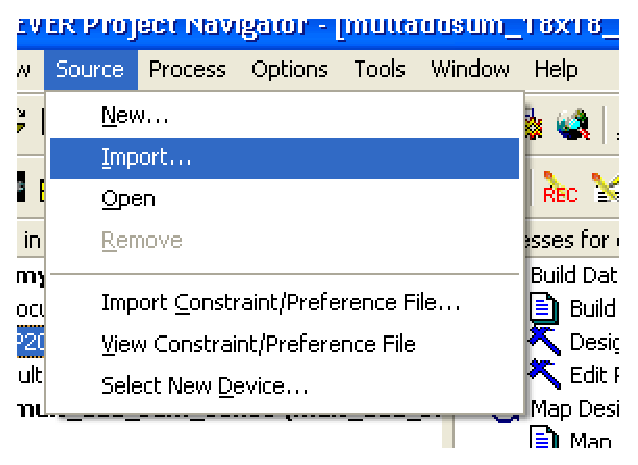
\includegraphics{bilder/sender/ispLeverimportfile.eps}
	\caption{VHDL-Datei importieren}
	\label{fig:ispLeverimportfile}
\end{figure}

\begin{figure}
	\centering
		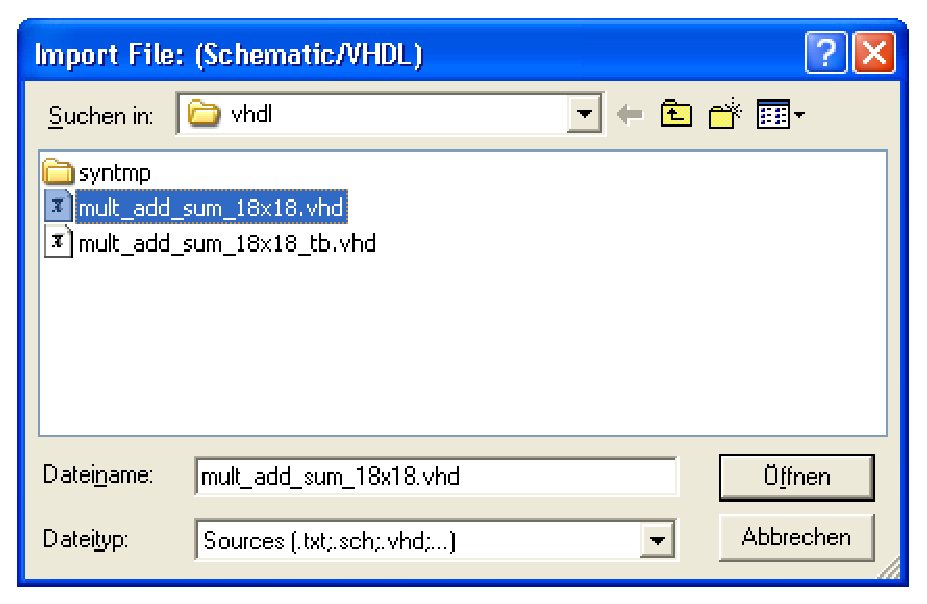
\includegraphics{bilder/sender/ispLeverimportdialog.eps}
	\caption{Importdialog}
	\label{fig:ispLeverimportdialog}
\end{figure}


\subsection[MODELSIM: Simulation mit zwei Signalgeneratoren]{MODELSIM: Simulation der Beschreibung mit zwei Signalgeneratoren}\label{subsec:modulator:sim}

\paragraph{Aufgabe 1.2:}

Simulieren Sie den zuvor erstellten Modulator mit Hilfe eines Digitalsignals, das von einem 4-Bit-PRN-Schieberegister mit XOR-Feedback �ber der letzten (MSB) Stufe \\
\verb|sv_prn_reg(3) <= sv_prn_reg(1) xor sv_prn_reg(0)|\\
erzeugt wird. Als Anfangsbelegung verwenden sie \verb|"1001"|. Der Schiebetakt soll bei etwa $1Hz$ liegen.

\paragraph{Aufgabe 2:}

Betrachten sie das modulierte Signal zu den Umschaltzeitpunkten genauer. Was stellen Sie fest?

\answergame{3}{Spr�nge im Ausgangssignal, die zu starken Oberwellen f�hren k�nnen.}

\subsection{VHDL: Modulator mit einem Signalgenerator}\label{subsec:modulator:HWdesc2}

\paragraph{Aufgabe 3:}
Verbessern Sie das Verhalten, indem Sie nur einen Signalgenerator verwenden und dessen Drehwinkel �ber einen Multiplexer ver�ndern.

\subsection[MODELSIM: Beschreibung mit einem Signalgenerator]{MODELSIM: Simulation der Beschreibung mit einem Signalgenerator}\label{subsec:modulator:sim2}

Simulieren Sie auch dies und kontrollieren nun das Verhalten im �bergangsbereich.

Was stellen sie bez�glich der Stetigkeit des Ausgangssignals fest?
\answergame{3}{Keine Spr�nge im Ausgangssignal}

Warum ist dies g�nstig f�r unsere Anwendung?
\answergame{4}{Keine Oberwellen, dadurch weniger St�rungen der Nachbarfrequenzen.}

\subsection{TEST: Praxistest}\label{subsec:modulator:test}

Testen Sie nun Ihren Entwurf auf der Hardware.
